\documentclass[11pt,fleqn]{article}

\setlength {\topmargin} {-.15in}
\setlength {\textheight} {8.6in}

\usepackage{amsmath}
\usepackage{amssymb}
\usepackage{color}
\usepackage{tikz}
\usetikzlibrary{automata,positioning,arrows}
\usepackage{diagbox}



\newcommand{\be}{\begin{enumerate}}
\newcommand{\ee}{\end{enumerate}}

\begin{document}

\textbf{Exercise 4.1.1:}: What is the maximum number of edges in a graph with V vertices and no parallel
edges? What is the minimum number of edges in a graph with V vertices, none of
which are isolated?\\

\textbf{Solution:}\\
Recall for $V$ vertices, there are ($V-1$) edges. 1st node connected to every node. 2nd node connected to every other node except first node, and so on. So start at ($V-1$) nodes and adding or counting this gives total number of edges.\\

ie; $V \thickspace + \thickspace (V-1) \thickspace + \thickspace (V-2) \thickspace + \thickspace (V-3) \thickspace + \thickspace ... \thickspace 1 \thickspace + 0$\\

We can also represent it using the following equation: $\frac{(v-1)(v)}{2}$ where v is the total number of vertices in the graph.

\begin{center}
	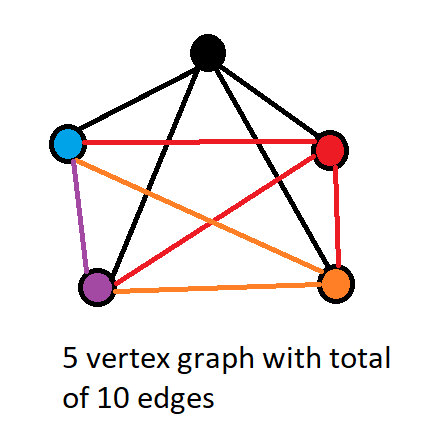
\includegraphics[scale=1]{4.1.1.png}
\end{center}

Now in terms of minimum number of edges, we just create a graph as a single line like a linkedlist. So $(v-1)$ edges as min. Recall a tree is a connected graph with NO CYCLES. So tree of size n has $n-1$ edges

\begin{center}
	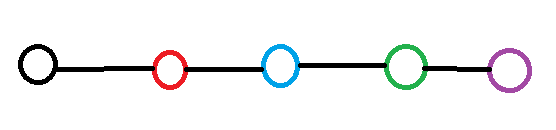
\includegraphics[scale=1]{4.1.1-soln.png}
\end{center}
	


\end{document}
